\documentclass[10pt,a4paper]{article}
\usepackage[margin=2.2cm]{geometry}
\usepackage{newtxtext,newtxmath}
\usepackage{graphicx}
\usepackage{booktabs,tabularx,multirow,makecell}
\usepackage{caption}
\usepackage{amsmath}
\usepackage{enumitem}
\usepackage[colorlinks=true,urlcolor=blue,linkcolor=black]{hyperref}
\captionsetup{font=small,labelfont=bf}
\hypersetup{pdftitle={Supplementary Material for TiDAL-Net (TII-26-8813)}}
\renewcommand{\thefigure}{S\arabic{figure}}
\renewcommand{\thetable}{S\arabic{table}}
\renewcommand{\thesection}{S\arabic{section}}
\renewcommand{\theequation}{S\arabic{equation}}
\setlength{\parskip}{0.35em}
\setlist[itemize]{leftmargin=1.5em,itemsep=1pt,topsep=2pt}

\title{Supplementary Material for\\
``A Time-Drift-Aware Liquid Spatio-Temporal Graph Network for Irregular Telemetry Reconstruction of Low Earth Orbit Satellites''}
\date{}

\begin{document}
\maketitle
\vspace{-2.5em}

\noindent Due to space limitations, only the key content is analyzed and described in the manuscript. This document collects the remaining supplementary material: the full experimental setup and degradation protocol (Section~\ref{sec:setup}), the detailed description and results of each experiment added in the revision (Sections~\ref{sec:low}--\ref{sec:sens}), the formulas of secondary steps that were moved from the method section of the manuscript (Section~\ref{sec:eqs}), and the contents of the GitHub repository (Section~\ref{sec:repo}). The document is available in the open-source repository given in footnote~2 of the manuscript, \url{https://github.com/Public-Model/TiDAL-Net}. Section, table, equation, and reference numbers without the prefix S refer to the revised manuscript. Unless stated otherwise, MAE is multiplied by $10^{2}$ and averaged over 30 runs.

\section{Experimental setup}
\label{sec:setup}

\subsection{Datasets}

Six telemetry datasets are used (Table~I of the manuscript). The public MSL, SMAP, and ESA-ADB datasets and the operational Real-A and Real-B datasets provide the primary single-stream evaluation, and Const-Sim is a supplementary multi-satellite extension. Table~\ref{tab:s1} lists the mission type of each dataset and its role. The ESA-ADB release anonymizes its missions and states only that they differ in purpose, orbit, and launch date, so no orbit is assigned to it. MSL and SMAP are used on their nominal one-minute grid, Const-Sim uses the simulated communication process of Section~II, and the native timing of ESA-ADB, Real-A, and Real-B is retained. Every dataset is split chronologically into training, validation, and test sets with a ratio of 6:2:2, and each split uses only its own reconstruction targets.

\begin{table}[!htbp]
\centering
\caption{Mission type of each dataset and its role in the evaluation.}
\label{tab:s1}
\small
\begin{tabularx}{0.88\linewidth}{l l X}
\toprule
Dataset & Mission type & Role \\
\midrule
SMAP & LEO & Primary LEO evidence, public benchmark \\
Real-A, Real-B & LEO & Primary LEO evidence, operational meteorological satellites \\
Const-Sim & LEO constellation & Supplementary multi-satellite extension with simulated links \\
MSL & Deep space (Mars rover) & General spacecraft benchmark, nominal one-minute grid \\
ESA-ADB & Not disclosed in the release & General spacecraft benchmark, native timing retained \\
\bottomrule
\end{tabularx}
\end{table}

\subsection{Degradation protocol and evaluated levels}

\textbf{Definitions.} Missing data are reference points without any received record. Timestamp-displaced samples are received records whose event time is offset by at least one nominal sampling interval. A displaced sample has been received and is never counted as missing, so the two parts do not overlap, and their sum gives the affected-data ratio. In the analyzed LEO telemetry, missing data account for 0.9\%--2.4\% of the reference points and displaced samples for 1.5\%--3.6\% of the received samples, and the affected-data ratio reaches about 5\%--6\%. This value describes routine LEO operation. Under severe conditions, the loss of LEO satellites can reach 10\% [2], [4]. Telemetry over longer links is also incomplete: losses of 2\% and 5\% were assumed in the analysis of a full-sky survey mission at the Sun--Earth L2 point [21], and the frame success rate of the NEAR spacecraft fell to 54\% at a Sun--Earth--probe angle of 1.3\textdegree{} near solar conjunction [22]. Table~\ref{tab:s3} relates the evaluated levels to these conditions.

\textbf{Ground truth.} Naturally missing telemetry has no ground truth. Part of the received normal data is therefore concealed and kept only as reconstruction targets, and the affected positions follow the irregularity statistics measured on ESA-ADB, Real-A, and Real-B rather than random deletion.

\textbf{Degradation types.} Both kinds of irregularity occur as isolated points and as consecutive runs. Lengths and magnitudes are drawn from distributions fitted to ESA-ADB, Real-A, and Real-B.
\begin{itemize}
\item \textit{Missing data:} isolated points; bursts of 2--8 samples; long gaps of 9 samples or more, drawn from the fitted tail of the gap-length distribution. Part of the bursts and long gaps are shared by several channels of one subsystem (correlated-channel loss). Over all gaps, the measured length has a median of one to two samples and a 95th percentile of 22 to 46 samples.
\item \textit{Timestamp displacement of at least one interval:} single offsets of 1--3 intervals; accumulated segments of 5--30 records, whose offset grows by 0.1--0.3 interval per record up to 4 intervals; blocks of 3--10 records with a constant offset of 1--2 intervals after a piecewise reset of the time mapping.
\item \textit{Sub-interval jitter:} offsets below one interval on 10\%--15\% of the received samples. These samples stay on their grid positions and are not counted in the affected-data ratio. Because most shifts are of this kind, the measured offset of all shifted records has a median of 0.3--0.4 intervals and a 95th percentile of 1.9--2.6 intervals.
\end{itemize}

\textbf{Composition of each level.} Table~\ref{tab:s2} and Fig.~\ref{fig:s1} give the dataset-averaged composition. At 3\%, 1.2\% of the grid positions are missing and 1.8\% are displaced, which keeps the proportion between the two parts measured in the LEO telemetry. As the level rises from 3\% to 10\%, the missing share increases from 40\% to 55\%, long gaps grow from 25\% to 44\% of the missing positions, and accumulated and reset offsets grow from 47\% to 62\% of the displaced positions. The isolated share of all affected positions falls from 71\% at 0.5\% to 31\% at 10\%. The degradation therefore grows mainly through bursts, long gaps, correlated loss, and accumulated offsets, which are the patterns that interrupt trend monitoring and cross-channel analysis in operation.

\begin{table}[!htbp]
\centering
\caption{Composition of the injected degradation at each level, averaged over the datasets. Missing and displaced shares are percentages of all grid positions; type shares are percentages within each part. Corr.: missing positions with correlated-channel loss; Iso.: share of all affected positions that are isolated.}
\label{tab:s2}
\small
\setlength{\tabcolsep}{4.5pt}
\begin{tabular}{ccccccccccc}
\toprule
\multirow{2}{*}{Level} & \multirow{2}{*}{Missing} & \multirow{2}{*}{Displaced} & \multicolumn{4}{c}{Missing types (\%)} & \multicolumn{3}{c}{Displacement types (\%)} & \multirow{2}{*}{Iso. (\%)} \\
\cmidrule(lr){4-7}\cmidrule(lr){8-10}
& & & Isolated & Burst & Long & Corr. & Single & Accum. & Reset & \\
\midrule
0.5\% & 0.2 & 0.3 & 68 & 22 & 10 & 9 & 73 & 20 & 7 & 71 \\
1.0\% & 0.4 & 0.6 & 64 & 24 & 12 & 11 & 69 & 22 & 9 & 67 \\
1.5\% & 0.6 & 0.9 & 59 & 26 & 15 & 13 & 66 & 24 & 10 & 63 \\
2.0\% & 0.8 & 1.2 & 55 & 27 & 18 & 15 & 63 & 26 & 11 & 60 \\
2.5\% & 1.0 & 1.5 & 50 & 29 & 21 & 16 & 58 & 29 & 13 & 55 \\
3\% & 1.2 & 1.8 & 45 & 30 & 25 & 18 & 53 & 32 & 15 & 50 \\
5\% & 2.0 & 3.0 & 38 & 32 & 30 & 22 & 48 & 35 & 17 & 44 \\
8\% & 4.0 & 4.0 & 30 & 32 & 38 & 27 & 42 & 38 & 20 & 36 \\
10\% & 5.5 & 4.5 & 25 & 31 & 44 & 31 & 38 & 40 & 22 & 31 \\
\bottomrule
\end{tabular}
\end{table}

\begin{table}[!htbp]
\centering
\caption{Correspondence between the evaluated affected-data ratios and on-orbit conditions.}
\label{tab:s3}
\small
\begin{tabularx}{0.88\linewidth}{c X}
\toprule
Level & Corresponding condition \\
\midrule
0.5\%--2.5\% & Very low orbits or well-covered links (Section~\ref{sec:low}) \\
3\% & LEO with light degradation \\
5\% & Routine LEO operation, about 5\%--6\% in the analyzed telemetry \\
8\% & Heavily degraded LEO links \\
10\% & Severe LEO conditions, up to 10\% [2], [4] \\
\midrule
Longer links & 2\%--5\% loss assumed for an L2 survey mission [21]; up to 46\% frame loss near solar conjunction [22]. The 3\%--10\% levels cover part of this range. \\
\bottomrule
\end{tabularx}
\end{table}

\begin{figure}[!htbp]
\centering
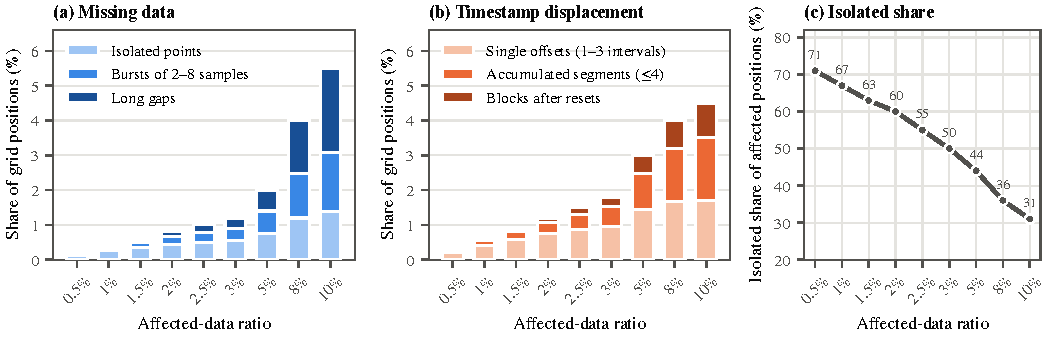
\includegraphics[width=\linewidth]{response_assets/R3_C2_composition.pdf}
\caption{Composition of the injected degradation. (a) Missing positions by type and (b) displaced positions by type, as percentages of all grid positions. (c) Share of all affected positions that are isolated points.}
\label{fig:s1}
\end{figure}

\subsection{Baselines, training, and implementation}

Fourteen baselines are compared: single-temporal models (Autoformer, PAREformer, MeaTS, SAITS), single-spatial models (GNN-DTAN, MSD-GNN), static spatio-temporal models (MAG, HiSTAR, MSTGAD, MAD-ODE, FuGLAD), and dynamic spatio-temporal models (TraverseNet, COOL, DSTGNN). The manuscript reports ten representative models, and the complete results of all fourteen are provided in the repository. All baselines keep their original backbones and are retrained for reconstruction. Forecasting models output the concealed segment instead of a future horizon, and detection models keep the prediction or reconstruction backbone without scoring, thresholding, or point adjustment. All methods share the same splits, affected positions, input and output lengths, training protocol, and metrics.

Comparative, ablation, and sensitivity experiments use affected-data ratios of 3\%, 5\%, 8\%, and 10\%. Each setting is repeated 30 times, and the paired results are compared with two-sided paired $t$-tests whose $p$-values are corrected by the Holm procedure. For a dataset with $M$ target channels, Bi-NSDE uses nine channel-wise feature stages with dimensions $[M,32M,64M,128M,256M,128M,64M,32M,M]$, and Li-GRU uses $[M,32M,64M,128M,64M,32M,M]$. The default settings are $S=10$, $P=8$, $\tau_{\min}=0.01$, $R_{\max}=3$, $W_{\mathrm{base}}=16$, $\lambda_{cc}=0.1$, $\gamma=0.3$, $K_{\mathrm{MIC}}=8$, $T_r=10$, $\gamma_t=0.1$, and $\Delta t_{\max}=10$, with time quantities in nominal intervals. TiDAL-Net is trained with Adam, a batch size of 16, a learning rate of $5\times10^{-4}$, up to 500 epochs, and an early-stopping patience of 50, on a workstation with two NVIDIA RTX 4080 GPUs and an Intel Core i9-14900KF processor.

\subsection{Evaluation metrics}

For the test target set $\Omega_{\mathrm{tar}}^{(\mathrm{te})}$, the accuracy metrics are
\begin{equation}
\mathrm{MAE}=\frac{1}{|\Omega_{\mathrm{tar}}^{(\mathrm{te})}|}\sum_{(i,k)\in\Omega_{\mathrm{tar}}^{(\mathrm{te})}}\left|\hat x_{i,k}-x^{\star}_{i,k}\right|,\qquad
\mathrm{RMSE}=\Bigg(\frac{1}{|\Omega_{\mathrm{tar}}^{(\mathrm{te})}|}\sum_{(i,k)\in\Omega_{\mathrm{tar}}^{(\mathrm{te})}}\left(\hat x_{i,k}-x^{\star}_{i,k}\right)^2\Bigg)^{1/2}.
\end{equation}
Efficiency is measured by trainable parameters, FLOPs, peak GPU memory, batch throughput, and single-window latency at batch size 1, which is the delay of one online reconstruction update. For the uncertainty analysis in Section~\ref{sec:unc}, the empirical coverage of the interval $\hat x_{i,k}\pm z_{\alpha}\sigma_{i,k}$ is the fraction of targets that fall inside it; the expected calibration error (ECE) is the mean absolute difference between nominal and empirical coverage over nominal levels from 10\% to 90\%; the Spearman correlation $\rho_s$ is computed between $\sigma_{i,k}$ and $|\hat x_{i,k}-x^{\star}_{i,k}|$; and the continuous ranked probability score (CRPS) is computed for the Gaussian predictive distribution with mean $\hat x_{i,k}$ and standard deviation $\sigma_{i,k}$.

\clearpage
\section{Low affected-data ratios (Comment 4)}
\label{sec:low}

\textbf{Purpose and setup.} This experiment examines whether time compensation still helps when the communication conditions are close to normal and whether it adds unnecessary computation. Levels of 0.5\%, 1.0\%, 1.5\%, 2.0\%, and 2.5\% are added below the 3\% level of the manuscript. They use the same degradation types as the other levels, and their composition is listed in Table~\ref{tab:s2}. COOL, DSTGNN, TiDAL-Net without Bi-NSDE, and TiDAL-Net are evaluated on all six datasets with 30 runs per level. To explain the ranking, the error is also broken down by position type: isolated positions, positions inside consecutive runs, and displaced samples. In addition, a preliminary gated inference is tested, in which Bi-NSDE is applied only to target positions and to the anchors and candidate neighbors that these positions require. Other valid observations are passed directly to Li-GRU with $\sigma_{i,k}=0$, and the same trained model is used.

\textbf{Results.} Table~\ref{tab:s4} and Fig.~\ref{fig:s2}(a) show that TiDAL-Net ranks second after COOL at 0.5\%--2.0\%, with MAE higher by 0.09, 0.07, 0.05, and 0.03, is level with COOL at 2.5\%, and is first again at 3.0\%. The differences are significant at 0.5\% and 1.0\% (Holm-adjusted $p<0.05$) but not at 1.5\%--2.5\%. Fig.~\ref{fig:s2}(b) shows that the difference between TiDAL-Net and COOL follows the isolated share: it decreases as the isolated share falls, crosses zero near 55\% (the 2.5\% level), and reaches $-0.62$ at 10\%. At the low levels, 55\%--71\% of the affected positions are isolated points, for which valid observations lie immediately on both sides and local interpolation is already accurate. Table~\ref{tab:s5} shows that TiDAL-Net still has 13.2\% and 18.8\% lower MAE than COOL on consecutive runs and displaced samples and the smallest run-to-run deviation, and removing Bi-NSDE increases its MAE by 5.0\%--10.0\%.

\textbf{Computation.} Bi-NSDE takes 2.6~ms of the 5.8~ms single-window latency at every ratio. Table~\ref{tab:s6} and Fig.~\ref{fig:s2}(d) show that the gated inference lowers the latency to 3.6--4.2~ms at 0.5\%--2.5\%, a reduction of 28\%--38\%, while the MAE changes by at most 0.01. Skipping valid positions removes small stochastic deviations but also removes the trajectories of observed neighbors that the drift uses as context, and the two effects nearly cancel. The gated inference is therefore reported as a preliminary result. Reliability-based activation of Bi-NSDE trained end to end, combined with a lightweight local estimator for isolated losses, is left for future work.

\begin{figure}[!htbp]
\centering
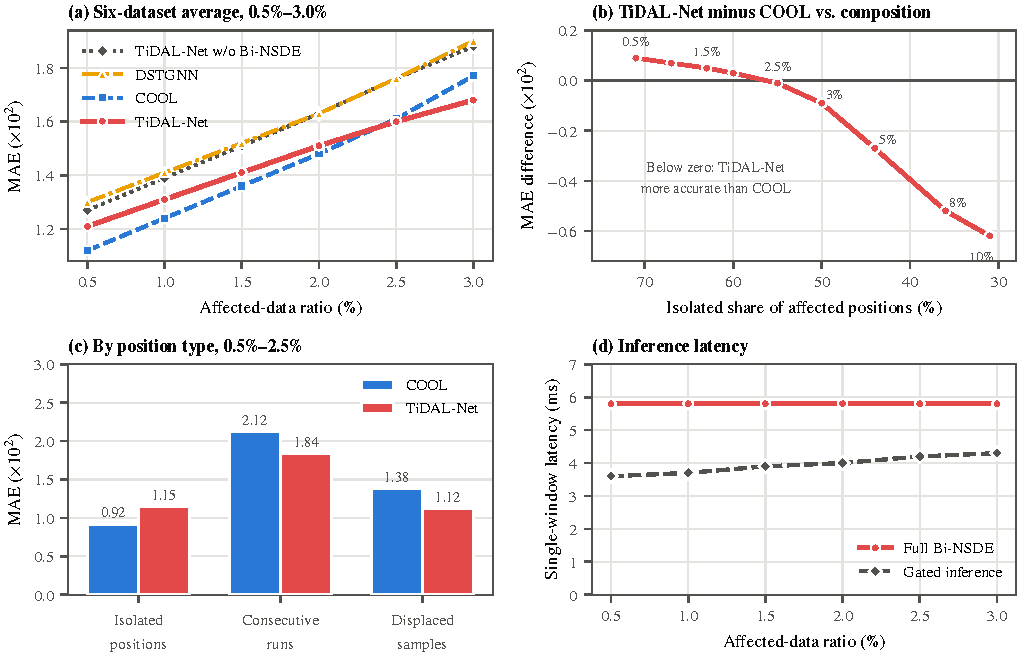
\includegraphics[width=0.92\linewidth]{response_assets/R3_C4_low_ratio.pdf}
\caption{Low affected-data ratios. (a) Six-dataset average MAE from 0.5\% to 3.0\%. (b) MAE difference between TiDAL-Net and COOL against the isolated share of each level from 0.5\% to 10\%; the 5\%--10\% values come from Table~II. (c) MAE by position type, averaged over 0.5\%--2.5\%. (d) Single-window latency with full Bi-NSDE and with the gated inference.}
\label{fig:s2}
\end{figure}

\begin{table}[!htbp]
\centering
\caption{MAE at low affected-data ratios, averaged over six datasets. The 3.0\% values of COOL, DSTGNN, and TiDAL-Net are the averages of Table~II.}
\label{tab:s4}
\small
\begin{tabular}{lcccccc}
\toprule
Method & 0.5\% & 1.0\% & 1.5\% & 2.0\% & 2.5\% & 3.0\% \\
\midrule
COOL & \textbf{1.12} & \textbf{1.24} & \textbf{1.36} & \textbf{1.48} & 1.61 & 1.77 \\
DSTGNN & 1.30 & 1.41 & 1.52 & 1.63 & 1.76 & 1.90 \\
TiDAL-Net w/o Bi-NSDE & 1.27 & 1.39 & 1.51 & 1.63 & 1.76 & 1.88 \\
TiDAL-Net & 1.21 & 1.31 & 1.41 & 1.51 & \textbf{1.60} & \textbf{1.68} \\
\midrule
Rank of TiDAL-Net & 2 & 2 & 2 & 2 & 1 & 1 \\
\bottomrule
\end{tabular}
\end{table}

\begin{table}[!htbp]
\centering
\caption{Error by position type and run-to-run standard deviation, averaged over 0.5\%--2.5\% and six datasets. Displaced samples are a subset of the affected positions.}
\label{tab:s5}
\small
\begin{tabular}{lcccc}
\toprule
Method & Isolated positions & Consecutive runs & Displaced samples & Std over 30 runs \\
\midrule
Share of affected positions (\%) & 55--71 & 29--45 & 60 & -- \\
COOL & \textbf{0.92} & 2.12 & 1.38 & 0.06--0.08 \\
TiDAL-Net & 1.15 & \textbf{1.84} & \textbf{1.12} & \textbf{0.04--0.05} \\
Difference (\%) & $+25.0$ & $-13.2$ & $-18.8$ & -- \\
\bottomrule
\end{tabular}
\end{table}

\begin{table}[!htbp]
\centering
\caption{Single-window latency (ms) and MAE of TiDAL-Net with full Bi-NSDE and with the gated inference.}
\label{tab:s6}
\small
\begin{tabular}{lcccccc}
\toprule
Quantity & 0.5\% & 1.0\% & 1.5\% & 2.0\% & 2.5\% & 3.0\% \\
\midrule
Latency, full & 5.8 & 5.8 & 5.8 & 5.8 & 5.8 & 5.8 \\
Latency, gated & 3.6 & 3.7 & 3.9 & 4.0 & 4.2 & 4.3 \\
MAE, full & 1.21 & 1.31 & 1.41 & 1.51 & 1.60 & 1.68 \\
MAE, gated & 1.20 & 1.30 & 1.41 & 1.51 & 1.60 & 1.67 \\
\bottomrule
\end{tabular}
\end{table}

\clearpage
\section{Long consecutive gaps and the no-anchor case (Comment 5)}
\label{sec:gap}

\textbf{Purpose and setup.} The gap lengths of the main evaluation follow the measured statistics, so long gaps appear only occasionally. This supplementary experiment isolates long interruptions and the case without valid anchors. On the five primary datasets, 5\% of the positions are set as missing and arranged into contiguous gaps of $G\in\{8,16,32,64,128\}$ nominal intervals. No timestamp displacement is added, so that the effect of gap length is isolated. The longest gap is about two hours for the one-minute datasets and three to six times the measured 95th-percentile gap. In the no-anchor case (NA), a channel is removed over the entire input window, so that Bi-NSDE has no valid anchor in either direction. In the harder case (NA+N), the candidate neighbors of that channel are removed at the same time, as in a subsystem-wide outage. SAITS, MAD-ODE, COOL, DSTGNN, and TiDAL-Net are compared, and the coverage of the scaled 90\% interval of TiDAL-Net is recorded inside the gaps.

\textbf{Results.} Table~\ref{tab:s7} and Fig.~\ref{fig:s3}(a) show that the error of every method grows with the gap length, but the curve of TiDAL-Net is the flattest. From $G=8$ to $G=128$, its MAE rises from 1.88 to 3.86, whereas that of COOL rises from 2.10 to 4.85, and the reduction relative to COOL increases from 10.5\% to 20.4\%. The two anchors bound each Bi-NSDE trajectory from both ends, the uncertainty-weighted fusion favors the closer or more certain direction, and the elapsed-time memory of Li-GRU keeps the slow trend across the gap. MAD-ODE also evolves in continuous time, but it has no bidirectional anchors or availability-aware neighbor screening, and its error grows faster. The real gaps of about 32--40 intervals in Figs.~5 and 6 of the manuscript lie in the middle of this range, and their behavior agrees with the $G=32$ point.

Without anchors, Bi-NSDE is inactive and the estimate relies on the Li-GRU state and on the neighbors retained by Li-GAT. TiDAL-Net still reduces MAE by 12.1\% relative to COOL, because the retained neighbors are screened by freshness and reachability. When the candidate neighbors are lost as well, the reduction falls to 3.6\%, and the output mainly follows the learned trend. Table~\ref{tab:s8} and Fig.~\ref{fig:s3}(c) show that the scaled uncertainty increases with gap length, while the coverage decreases slightly to 86.4\% at $G=128$, so estimates inside long outages should be interpreted together with their uncertainty. Prior information from subsystem models is a possible remedy for such outages.

\begin{figure}[!htbp]
\centering
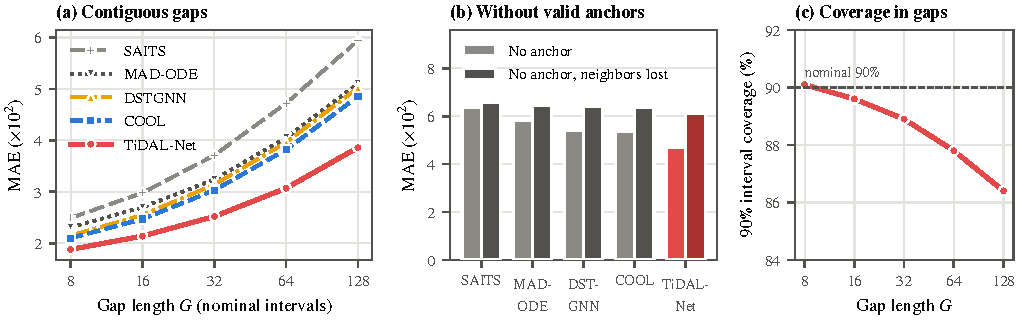
\includegraphics[width=\linewidth]{response_assets/R3_C5_long_gap.pdf}
\caption{Long consecutive gaps. (a) MAE versus gap length. (b) MAE without valid anchors, and when the candidate neighbors are also lost (darker bars). (c) Coverage of the scaled 90\% interval of TiDAL-Net inside the gaps.}
\label{fig:s3}
\end{figure}

\begin{table}[!htbp]
\centering
\caption{MAE under contiguous gaps, averaged over the five primary datasets. NA: no valid anchor; NA+N: no valid anchor, with the candidate neighbors also lost.}
\label{tab:s7}
\small
\begin{tabular}{lccccccc}
\toprule
Method & $G=8$ & $G=16$ & $G=32$ & $G=64$ & $G=128$ & NA & NA+N \\
\midrule
SAITS & 2.49 & 2.98 & 3.71 & 4.72 & 5.94 & 6.37 & 6.58 \\
MAD-ODE & 2.31 & 2.70 & 3.24 & 4.05 & 5.10 & 5.82 & 6.47 \\
COOL & 2.10 & 2.47 & 3.03 & 3.82 & 4.85 & 5.36 & 6.35 \\
DSTGNN & 2.15 & 2.55 & 3.14 & 3.96 & 5.02 & 5.41 & 6.41 \\
TiDAL-Net & \textbf{1.88} & \textbf{2.14} & \textbf{2.52} & \textbf{3.07} & \textbf{3.86} & \textbf{4.71} & \textbf{6.12} \\
\midrule
Reduction vs. COOL (\%) & 10.5 & 13.4 & 16.8 & 19.6 & 20.4 & 12.1 & 3.6 \\
\bottomrule
\end{tabular}
\end{table}

\begin{table}[!htbp]
\centering
\caption{Scaled uncertainty of TiDAL-Net within the gaps. The mean $\sigma_{i,k}$ is on the same $\times10^{2}$ scale as MAE.}
\label{tab:s8}
\small
\begin{tabular}{lccccc}
\toprule
Quantity & $G=8$ & $G=16$ & $G=32$ & $G=64$ & $G=128$ \\
\midrule
Mean scaled $\sigma_{i,k}$ ($\times10^{2}$) & 2.4 & 2.7 & 3.2 & 3.8 & 4.6 \\
90\% coverage (\%) & 90.1 & 89.6 & 88.9 & 87.8 & 86.4 \\
\bottomrule
\end{tabular}
\end{table}

\clearpage
\section{Reliability of the estimated uncertainty (Comment 3)}
\label{sec:unc}

\textbf{Purpose and setup.} The uncertainty $\sigma_{i,k}$ is used in the directional fusion, in the reliability $r_{i,k}$ and the input of Li-GRU, and in the node feature of Li-GAT, and it can be reported with each reconstruction. This experiment tests whether it reflects the error of the final reconstruction $\hat x_{i,k}$. The interval $\hat x_{i,k}\pm1.645\sigma_{i,k}$ is treated as a nominal 90\% Gaussian interval. Because $\sigma_{i,k}$ is produced by Bi-NSDE before Li-GRU and Li-GAT refine the estimate, one positive scale per dataset is fitted on the validation split by minimizing the Gaussian negative log-likelihood of the final residuals and then kept fixed for testing. Coverage, ECE, the Spearman correlation with the absolute error (also within bins of equal anchor distance, which removes the part explained by elapsed time alone), and a sparsification test that removes the 10\% most uncertain positions are computed. Positions without a valid anchor (0.6\%--1.9\% of the targets) have no path dispersion and are treated in Section~\ref{sec:gap}. CSDI and TiDAL-Net without diffusion are compared with the same validation scaling.

\textbf{Results.} Table~\ref{tab:s9} and Fig.~\ref{fig:s4}(a)--(b) show a Spearman correlation of 0.63--0.73, which remains 0.41--0.56 within equal anchor-distance bins, so $\sigma_{i,k}$ is not merely a function of elapsed time. Removing the 10\% most uncertain positions lowers MAE by 21.4\%--27.9\%. Raw intervals are conservative on MSL, SMAP, Real-A, and Real-B and under-cover ESA-ADB and Const-Sim. The under-coverage is concentrated after piecewise timestamp resets in ESA-ADB and after link reselection in Const-Sim: within five intervals after a reset in ESA-ADB, the raw coverage is 81.6\%. With fitted scales of 0.87--1.07, the coverage becomes 89.1\%--90.6\%, and ECE falls to 0.8\%--1.4\%. After scaling, the coverage is 90.4\% for positions with two valid anchors and 88.6\% for positions with one. Table~\ref{tab:s10} and Fig.~\ref{fig:s4}(c) show that, at similar coverage, the intervals of TiDAL-Net are about 28\% narrower than those of CSDI and its CRPS is lower. Without diffusion, the correlation drops to 0.35 on average and the coverage stays at 85.6\% even after scaling, so the diffusion term is the main source of the information in $\sigma_{i,k}$. Replacing the uncertainty term of the fusion weight with the anchor-distance term alone increases the average MAE by 5.8\%, compared with 10.3\% for the unweighted mean fusion in Table~III.

\begin{figure}[!htbp]
\centering
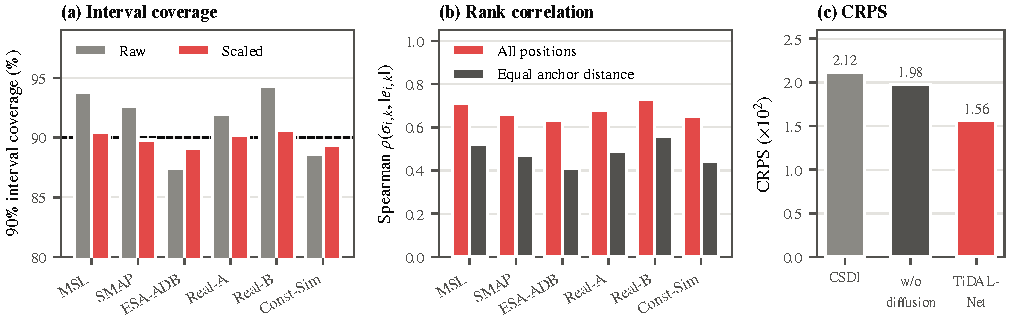
\includegraphics[width=\linewidth]{response_assets/R3_C3_uncertainty.pdf}
\caption{Reliability of the estimated uncertainty. (a) Coverage of the nominal 90\% interval before and after scaling. (b) Spearman correlation between $\sigma_{i,k}$ and the absolute error over all positions and within equal anchor-distance bins. (c) CRPS of CSDI, TiDAL-Net without diffusion, and TiDAL-Net.}
\label{fig:s4}
\end{figure}

\begin{table}[!htbp]
\centering
\caption{Reliability of $\sigma_{i,k}$, averaged over four affected-data ratios. $\rho_s^{\mathrm{bin}}$: Spearman correlation within equal anchor-distance bins; $s$: fitted scale; $\Delta$MAE: MAE reduction after removing the 10\% most uncertain positions.}
\label{tab:s9}
\small
\begin{tabular}{lcccccccc}
\toprule
Dataset & $\rho_s$ & $\rho_s^{\mathrm{bin}}$ & Cov. raw (\%) & Cov. scaled (\%) & ECE raw (\%) & ECE scaled (\%) & $s$ & $\Delta$MAE (\%) \\
\midrule
MSL & 0.71 & 0.52 & 93.8 & 90.4 & 3.1 & 0.9 & 0.89 & 25.3 \\
SMAP & 0.66 & 0.47 & 92.6 & 89.8 & 2.7 & 1.1 & 0.92 & 23.1 \\
ESA-ADB & 0.63 & 0.41 & 87.4 & 89.1 & 3.6 & 1.4 & 1.07 & 21.4 \\
Real-A & 0.68 & 0.49 & 91.9 & 90.2 & 2.2 & 0.8 & 0.95 & 24.6 \\
Real-B & 0.73 & 0.56 & 94.3 & 90.6 & 3.4 & 1.0 & 0.87 & 27.9 \\
Const-Sim & 0.65 & 0.44 & 88.6 & 89.3 & 3.0 & 1.3 & 1.05 & 22.2 \\
\bottomrule
\end{tabular}
\end{table}

\begin{table}[!htbp]
\centering
\caption{Comparison of uncertainty quality, averaged over six datasets and four affected-data ratios. Coverage and ECE are after scaling; MAE, interval width, and CRPS are multiplied by $10^{2}$.}
\label{tab:s10}
\small
\begin{tabular}{lcccccc}
\toprule
Method & MAE & $\rho_s$ & 90\% coverage (\%) & ECE (\%) & Interval width & CRPS \\
\midrule
CSDI & 3.02 & 0.58 & 90.8 & 1.6 & 12.6 & 2.12 \\
TiDAL-Net w/o diffusion & 2.72 & 0.35 & 85.6 & 4.8 & 7.4 & 1.98 \\
TiDAL-Net & \textbf{2.20} & \textbf{0.68} & 89.9 & \textbf{1.1} & 9.1 & \textbf{1.56} \\
\bottomrule
\end{tabular}
\end{table}

\clearpage
\section{Mission-mode shift (Comment 1)}
\label{sec:shift}

\textbf{Purpose and setup.} The candidate graph $\mathcal E^{(0)}$ is estimated on the training split, and Li-GAT can prune and reweight its edges but cannot create new ones. This experiment quantifies the effect of relations that appear only in mission modes absent from training. For Real-A and Real-B, orbit-control and payload-calibration periods are removed from the training and validation splits and appear only in the test set. For Const-Sim, the SAR imaging mode with intersatellite relay is withheld in the same way. The candidate graph is rebuilt without these modes and the model is retrained, and the analysis focuses on the channel relations that occur only in the withheld modes. Fixed GAT, COOL, and DSTGNN are evaluated under the same data split. Two variants of TiDAL-Net are included: a dense candidate graph that allows all channel pairs, and a reference that rebuilds $\mathcal E^{(0)}$ with the withheld modes included. Strong pairs are channel pairs with $\mathrm{MIC}\ge\gamma$ on the unseen-mode reference.

\textbf{Results.} Table~\ref{tab:s11} and Fig.~\ref{fig:s5}(a) show that all graph-based methods degrade on the unseen modes. The average MAE of TiDAL-Net increases by 23.5\%, close to 23.4\% for COOL and 21.0\% for DSTGNN, and its unseen-mode MAE of 2.33 remains the lowest among the default models. Fixed GAT, which uses the same MIC graph without online pruning and reweighting, degrades by 29.7\%. Table~\ref{tab:s12} and Fig.~\ref{fig:s5}(b) show that 6.1\%--11.8\% of the strong pairs are absent from $\mathcal E^{(0)}$ and that the increase concentrates on the channels in these pairs (41.6\% versus 14.3\%). The rebuilt-graph reference lowers the unseen-mode MAE from 2.33 to 2.06, so about 61\% of the increase is attributable to the absent relations. The dense candidate graph reaches 2.21 but raises the seen-mode MAE by 6.2\% and the latency from 5.8 to 9.6~ms. Pruning and reweighting thus follow changes in the strength or availability of known relations, whereas a coupling absent from training cannot be represented until $\mathcal E^{(0)}$ is re-estimated from verified telemetry of the new mode.

\begin{figure}[!htbp]
\centering
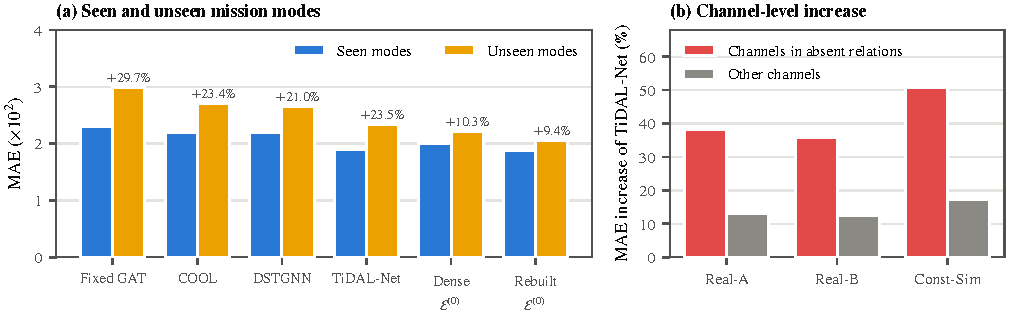
\includegraphics[width=\linewidth]{response_assets/R3_C1_mode_shift.pdf}
\caption{Mission-mode shift. (a) Seen-mode and unseen-mode MAE averaged over Real-A, Real-B, and Const-Sim. (b) MAE increase of TiDAL-Net on channels involved in relations absent from $\mathcal E^{(0)}$ and on the other channels.}
\label{fig:s5}
\end{figure}

\begin{table}[!htbp]
\centering
\caption{Seen (S) and unseen (U) mode MAE at the 5\% ratio. The increase is computed on the average over the three datasets.}
\label{tab:s11}
\small
\begin{tabular}{lcccccccc}
\toprule
\multirow{2}{*}{Method} & \multicolumn{2}{c}{Real-A} & \multicolumn{2}{c}{Real-B} & \multicolumn{2}{c}{Const-Sim} & \multirow{2}{*}{Increase (\%)} & \multirow{2}{*}{Latency (ms)} \\
& S & U & S & U & S & U & & \\
\midrule
Fixed GAT & 2.93 & 3.79 & 1.45 & 1.88 & 2.53 & 3.29 & 29.7 & 5.2 \\
COOL & 3.04 & 3.71 & 1.27 & 1.57 & 2.26 & 2.83 & 23.4 & 3.07 \\
DSTGNN & 2.95 & 3.56 & 1.37 & 1.66 & 2.26 & 2.74 & 21.0 & 2.84 \\
TiDAL-Net & 2.74 & 3.31 & 1.17 & 1.45 & 1.76 & 2.24 & 23.5 & 5.8 \\
Dense $\mathcal E^{(0)}$ & 2.86 & 3.18 & 1.25 & 1.38 & 1.91 & 2.08 & 10.3 & 9.6 \\
Rebuilt $\mathcal E^{(0)}$ & 2.73 & 2.95 & 1.17 & 1.30 & 1.75 & 1.93 & 9.4 & 5.9 \\
\bottomrule
\end{tabular}
\end{table}

\begin{table}[!htbp]
\centering
\caption{Relations absent from the default candidate graph in the unseen modes and the MAE increase of TiDAL-Net.}
\label{tab:s12}
\small
\begin{tabular}{lccc}
\toprule
Dataset & Strong pairs absent (\%) & Channels in absent pairs (\%) & Other channels (\%) \\
\midrule
Real-A & 7.4 & 38.2 & 13.1 \\
Real-B & 6.1 & 35.7 & 12.6 \\
Const-Sim & 11.8 & 50.9 & 17.2 \\
Average & 8.4 & 41.6 & 14.3 \\
\bottomrule
\end{tabular}
\end{table}

\clearpage
\section{Sensitivity of the graph-related parameters (Comment 6)}
\label{sec:sens}

\textbf{Purpose and setup.} Five parameters of the candidate and dynamic graphs are added to the sensitivity analysis: the MIC threshold $\gamma$ and the neighbor count $K_{\mathrm{MIC}}$ in Eq.~(22), which define the candidate graph; the reliability decay constant $T_r$ in $r_j(t)$, which is used in Eq.~(8) and in the Li-GRU input; the historical decay rate $\gamma_t$ in Eq.~(25); and the information freshness threshold $\Delta t_{\max}$ in Eq.~(27). The defaults are $\gamma=0.3$, $K_{\mathrm{MIC}}=8$, $T_r=10$, $\gamma_t=0.1$, and $\Delta t_{\max}=10$, with time quantities in nominal intervals. Each parameter is varied over six values with 30 repetitions while the other settings are fixed. Because Eq.~(27) applies $\Delta t_{\max}$ only between channels on different satellites, $\Delta t_{\max}$ is evaluated on Const-Sim, and the other parameters are averaged over six datasets and four affected-data ratios.

\textbf{Results.} Table~\ref{tab:s13} and Fig.~\ref{fig:s6} show a flat region around every default. MAE stays within 0.0220--0.0232 for $\gamma=0.2$--$0.5$ and $K_{\mathrm{MIC}}=6$--$16$. A smaller $\gamma$ or a larger $K_{\mathrm{MIC}}$ admits weak relations and raises the latency to 7.1~ms at $\gamma=0.1$ and 8.1~ms at $K_{\mathrm{MIC}}=24$ without improving accuracy, whereas a larger $\gamma$ or a smaller $K_{\mathrm{MIC}}$ removes useful relations. $T_r=5$--$50$ and $\gamma_t=0.05$--$0.5$ keep MAE below 0.0230; faster decay discards valid neighbors, and slower decay keeps stale ones. On Const-Sim, $\Delta t_{\max}=5$--$40$ keeps MAE within 0.0210--0.0221, whereas removing the threshold gives 0.0236 because outdated cross-satellite states are used during link reselection. Over these ranges, the MAE stays within about 5\% of the default.

\begin{table}[!htbp]
\centering
\caption{Sensitivity of the graph-related parameters. Defaults are underlined; latency is in ms and is 5.8~ms for parameters without a latency row.}
\label{tab:s13}
\small
\begin{tabular}{llcccccc}
\toprule
Parameter & Quantity & \multicolumn{6}{c}{Evaluated values} \\
\midrule
\multirow{3}{*}{$\gamma$} & Value & 0.1 & 0.2 & \underline{0.3} & 0.4 & 0.5 & 0.6 \\
& MAE & 0.0231 & 0.0224 & \textbf{0.0220} & 0.0223 & 0.0232 & 0.0247 \\
& Latency & 7.1 & 6.3 & 5.8 & 5.5 & 5.3 & 5.1 \\
\midrule
\multirow{3}{*}{$K_{\mathrm{MIC}}$} & Value & 4 & 6 & \underline{8} & 12 & 16 & 24 \\
& MAE & 0.0238 & 0.0226 & \textbf{0.0220} & 0.0221 & 0.0225 & 0.0233 \\
& Latency & 5.1 & 5.4 & 5.8 & 6.4 & 7.0 & 8.1 \\
\midrule
\multirow{2}{*}{$T_r$} & Value & 2 & 5 & \underline{10} & 20 & 50 & 100 \\
& MAE & 0.0243 & 0.0227 & \textbf{0.0220} & 0.0222 & 0.0229 & 0.0236 \\
\midrule
\multirow{2}{*}{$\gamma_t$} & Value & 0.01 & 0.05 & \underline{0.1} & 0.2 & 0.5 & 1.0 \\
& MAE & 0.0230 & 0.0223 & \textbf{0.0220} & 0.0222 & 0.0229 & 0.0241 \\
\midrule
\multirow{2}{*}{$\Delta t_{\max}$} & Value & 2 & 5 & \underline{10} & 20 & 40 & $\infty$ \\
& MAE & 0.0232 & 0.0217 & \textbf{0.0210} & 0.0213 & 0.0221 & 0.0236 \\
\bottomrule
\end{tabular}
\end{table}

\begin{figure}[!htbp]
\centering
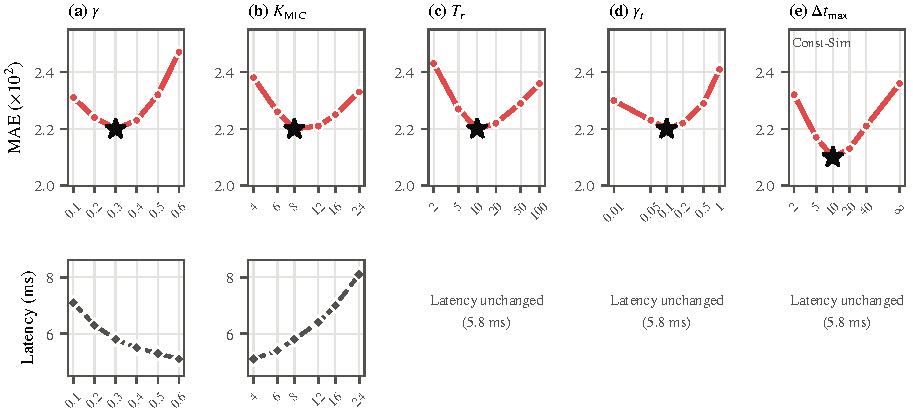
\includegraphics[width=\linewidth]{response_assets/R3_C6_sensitivity.pdf}
\caption{Sensitivity of the graph-related parameters. Top row: MAE of (a) $\gamma$, (b) $K_{\mathrm{MIC}}$, (c) $T_r$, (d) $\gamma_t$, and (e) $\Delta t_{\max}$ (Const-Sim), with the default marked by a star. Bottom row: latency for the two parameters that change the candidate graph size.}
\label{fig:s6}
\end{figure}

\clearpage
\section{Formulas of secondary steps moved from the manuscript}
\label{sec:eqs}

To keep the manuscript within the page limit, the formulas below were moved from the method section. They restate definitions or standard expressions; every variable they introduce is also defined in the text of the manuscript, and the key steps of TiDAL-Net remain in the manuscript.

\textbf{Normalized event time and input mask} (Section~III-A, after Eq.~(1)). The onboard event epoch is normalized to mission elapsed time in nominal intervals, and the input mask marks valid observations on the grid:
\begin{equation}
\tilde t_{i,q}=\frac{a_{i,q}-a_{i,0}}{\Delta^{\mathrm{nom}}},\qquad m^{\mathrm{in}}_{i,k}\in\{0,1\}.
\end{equation}

\textbf{Sources of irregularity} (Section~III-A, after Eq.~(4)). Event intervals are non-uniform, the ground receiving time adds a path-dependent delay and a residual uncertainty to the event epoch, and the input masks of channels in the same subsystem are correlated:
\begin{gather}
\tilde t_{i,q}-\tilde t_{i,q-1}\neq\mathrm{const},\\
t^{\mathrm{rec}}_{i,q}=a_{i,q}+\Lambda_{\pi_{n(i)}}\!\left(a_{i,q}\right)+\eta^{\mathrm{rec}}_{i,q},\\
\operatorname{Cov}\!\left(m^{\mathrm{in}}_{i,k},m^{\mathrm{in}}_{j,k}\right)\neq0,\qquad i,j\in\mathcal I_{\mathrm{sub}},
\end{gather}
where $\Lambda_{\pi_{n}}$ is the delay along the communication path $\pi_n$ of satellite $n$ and $\eta^{\mathrm{rec}}_{i,q}$ is the residual receiving-time uncertainty. The onboard event time is unchanged.

\textbf{Integral form of Bi-NSDE} (Section~III-B, after Eq.~(7)). The latent trajectory of Eqs.~(6) and (7) is the It\^o process
\begin{equation}
\mathbf h^{(\mathrm D)}_{i,k}(s)=\mathbf h^{(\mathrm D)}_{i,k}(0)+\int_0^s f^{(\mathrm D)}_{\theta}\!\left(\mathbf h^{(\mathrm D)}_{i,k}(u),\mathbf c^{(\mathrm D)}_{i,k}(u),\chi^{(\mathrm D)}_{i,k}(u),\mathbf e_i\right)\mathrm du+\int_0^s g^{(\mathrm D)}_{\phi}\!\left(\mathbf h^{(\mathrm D)}_{i,k}(u),\chi^{(\mathrm D)}_{i,k}(u),\mathbf e_i\right)\odot\mathrm d\mathbf W^{(\mathrm D)}_{i,k}(u),
\end{equation}
which has a unique strong solution under standard Lipschitz and linear-growth conditions and is discretized by the Euler--Maruyama update in Eq.~(9).

\textbf{Continuous-time form of Li-GRU} (Section~III-C, with Eqs.~(17)--(20)). During $(t_{k-1},t_k]$, the gates $\mathbf z_{i,k}$, the candidate state $\tilde{\mathbf h}_{i,k}$, and the time constant $\boldsymbol\tau_{i,k}$ are fixed, and the hidden state follows the first-order relaxation
\begin{equation}
\frac{\mathrm d\mathbf h_i}{\mathrm dt}=\mathbf z_{i,k}\odot\left(\tilde{\mathbf h}_{i,k}-\mathbf h_i\right)\oslash\boldsymbol\tau_{i,k},\qquad \mathbf h_i(t_{k-1})=\mathbf h^{+}_{i,k-1}.
\end{equation}
Because the equation is linear and elementwise with constant coefficients, its solution at $t_k$ is
\begin{equation}
\mathbf h_i(t_k)=\tilde{\mathbf h}_{i,k}+\left(\mathbf h^{+}_{i,k-1}-\tilde{\mathbf h}_{i,k}\right)\odot\exp\!\left[-(t_k-t_{k-1})\,\mathbf z_{i,k}\oslash\boldsymbol\tau_{i,k}\right]
=\boldsymbol\vartheta_{i,k}\odot\mathbf h^{+}_{i,k-1}+\left(\mathbf 1_H-\boldsymbol\vartheta_{i,k}\right)\odot\tilde{\mathbf h}_{i,k},
\end{equation}
which is Eqs.~(19) and (20). A long interval or a small time constant drives $\boldsymbol\vartheta_{i,k}$ toward zero and the state toward the candidate, whereas a short interval or a large time constant retains the previous state.

\textbf{Node feature, history window, and state similarity} (Section~III-D). The node feature used by Li-GAT, the history window of length $L_{i,k}$ in Eqs.~(25) and (26), and the cosine similarity used in Eq.~(28) are
\begin{gather}
\mathbf v_{i,k}=\left[\mathbf h_{i,k}^{\top},\bar x_{i,k},\sigma_{i,k},r_{i,k},\mathbf e_i^{\top}\right]^{\top}\in\mathbb R^{H+E+3},\\
\mathcal W_{i,k}=\left\{k'\;\middle|\;\max(1,k-L_{i,k}+1)\le k'\le k\right\},\\
\varsigma_{ij,k}=\frac{\mathbf v_{i,k}^{\top}\bar{\mathbf v}^{(i)}_{j,k}}{\|\mathbf v_{i,k}\|_2\,\|\bar{\mathbf v}^{(i)}_{j,k}\|_2+\varepsilon}.
\end{gather}

\textbf{Reconstruction losses} (Section~III-E, in Eq.~(33)). The squared and absolute reconstruction terms are computed over the training targets:
\begin{equation}
\mathcal L_{\mathrm{rec}}=\frac{1}{|\Omega^{(\mathrm{tr})}_{\mathrm{tar}}|}\sum_{(i,k)\in\Omega^{(\mathrm{tr})}_{\mathrm{tar}}}\left(\hat x_{i,k}-x^{\star}_{i,k}\right)^2,\qquad
\mathcal L_{\mathrm{abs}}=\frac{1}{|\Omega^{(\mathrm{tr})}_{\mathrm{tar}}|}\sum_{(i,k)\in\Omega^{(\mathrm{tr})}_{\mathrm{tar}}}\left|\hat x_{i,k}-x^{\star}_{i,k}\right|.
\end{equation}

\clearpage
\section{Contents of the GitHub repository}
\label{sec:repo}

The supplementary files are placed in the open-source repository \url{https://github.com/Public-Model/TiDAL-Net} together with the demonstration code and the complete results of the manuscript:
\begin{itemize}
\item \texttt{Supplementary\_Material.pdf}: this document.
\item \texttt{supplementary/figures/}: Figs.~S1--S6 as 600-dpi PNG files and as vector PDF, SVG, and EMF files.
\item \texttt{supplementary/data/}: the values of Tables~S1--S13 and of the curves in Figs.~S1--S6 as CSV files.
\item \texttt{supplementary/equations.pdf}: Section~\ref{sec:eqs} of this document as a separate file.
\item \texttt{supplementary/source/}: the \LaTeX{} source of this document and the Python script that draws Figs.~S1--S6.
\end{itemize}

\end{document}
